\documentclass[11pt,a4paper,twoside,headsepline,numbers=noenddot,toc=bibliography,cleardoublepage=empty,parskip=half,DIV=calc,BCOR=6mm,pagesize=pdftex]{article}



%---------------------------------------------------------
%	Speed up compile time
%---------------------------------------------------------
% uncommenting these lines will disable PDF compression.
% As a result the PDF will be massive (~100MB) but will compile faster.
% Make sure to comment this out when you want to share the PDF.

% \pdfcompresslevel=0
% \pdfobjcompresslevel=0


%---------------------------------------------------------
%	Aditional Packages
%---------------------------------------------------------
\usepackage[german]{babel}
\usepackage{titlepage} % included in the archive and does some styling
\usepackage[absolute]{textpos}
\usepackage[separate-uncertainty = true]{siunitx} % enable easy SI units with \SI{VALUE}{\meter}
% Note: errors are written like this \SI{10(1)}{\meter} will show up as (10 ± 1) m

\usepackage{subcaption} % To have multiple plots side by side
\usepackage{float}
\usepackage{url} % enable clickable URLs
\usepackage{listings} % to have code blocks in your document
\usepackage{xcolor}
\usepackage{doi}
\usepackage{microtype}
\usepackage{booktabs}
\usepackage{nicefrac} % creates a fraction that is nicer when used in text \nicefrac{1}{2}
\usepackage[acronym]{glossaries} % creates list of acronyms for you and handles everything

% Make acronyms and tell it the file with the acronym definitions
\makenoidxglossaries

% Maybe you will need some of these, therefore I have not removed them!
% -----------------------
%     Theory part
% -----------------------
\newacronym{snrs}{SNRs}{Supernova Remnants}
\newacronym{ams}{AMS-02}{Alpha Magnetic Spectrometer}
\newacronym{fermilat}{Fermi-LAT}{Fermi Large Area Telescope}
\newacronym{hegra}{HEGRA}{High Energy Gamma Ray Astronomy}
\newacronym{pwn}{PWN}{Pulsar Wind Nebula}
\newacronym{pwne}{PWNe}{Pulsar Wind Nebulae}

\newacronym{hess}{H.E.S.S.}{High Energy Stereoscopic System}
\newacronym{dc}{DC}{Davies-Cotton}
\newacronym{ars}{ARS}{Analogue Ring Samplers}
\newacronym{fov}{FoV}{Field of View}
\newacronym{cta}{CTA}{Cherenkov Telescope Array}
\newacronym{nsb}{NSB}{Night Sky Background}
\newacronym{cog}{CoG}{Centre of Gravity}
\newacronym{adc}{ADC}{Analogue to Digital Converter}

\newacronym{psf}{PSF}{Point Spread Function}
\newacronym{pe}{p.e.}{Photo Electron}
\newacronym{ism}{ISM}{Interstellar Medium}
\newacronym{gzk}{GZK}{Greisen–Zatsepin–Kuzmin}
\newacronym{cmb}{CMB}{Cosmic Microwave Background}
\newacronym{dsa}{DSA}{Diffusive Shock Acceleration}
\newacronym{grbs}{GRBs}{Gamma Ray Bursts}
\newacronym{agn}{AGN}{Active Galactic Nuclei}
\newacronym{sbgs}{SBGs}{Starburst Galaxies}
\newacronym{ic}{IC}{Inverse Compton}
\newacronym{kn}{KN}{Klein-Nishina}
\newacronym{hawc}{HAWC}{High-Altitude Water Cherenkov Observatory}

\newacronym{eas}{EAS}{Extensive Air Showers}
% -----------------------
%     Corsika simtel
% -----------------------
\newacronym{kascade}{KASCADE}{Karlsruhe Shower Core and Array Detector}
\newacronym{egs4}{EGS4}{Electron Gamma Shower system 4}
\newacronym{venus}{VENUS}{Very Energetic NUclear Scattering}
\newacronym{qgsjet}{QGSJET}{Quark Gluon String model with JETs}
\newacronym{dmpjet}{DMPJET}{Dual Parton Model with JETs}
\newacronym{urqmd}{UrQMD}{Ultra relativistic Quantum Molecular Dynamics}


% -----------------------
%     CTA
% -----------------------
\newacronym{lsts}{LSTs}{Large-Sized Telescopes}
\newacronym{msts}{MSTs}{Medium-Sized Telescopes}
\newacronym{ssts}{SSTs}{Small-Sized Telescopes}
\newacronym{vhe}{VHE}{Very High Energy}
\newacronym{checs}{CHEC-S}{Compact High Energy Camera with Silicon \acrshort{pmts}}
\newacronym{asic}{ASIC}{Application Specific Integrated Circuit}
\newacronym{sipm}{SiPM}{Silicon Photomultiplier}
\newacronym{tf}{TF}{Transfer Function}
% Large-Sized telescopes 

\newacronym{tm}{TM}{TARGET-Module}
\newacronym{target}{TARGET}{TeV Array Readout electronics with GSa/s sampling and Event Trigger}
\newacronym{bdt}{BDT}{Boosted Decision Tree}
\newacronym{ct5tea}{CT5TEA}{CTA-TARGET-5TEA version}
\newacronym{ctc}{CTC}{CTA-TARGET-C version}

\newacronym{impact}{ImPACT}{Image Pixel-wise fit for Atmospheric Cherenkov Telescopes}
\newacronym{sc}{SC}{Schwarzschild-Couder}

\newacronym{corsika}{CORSIKA}{Cosmic Ray Simulations for Kascade}
\newacronym{iact}{IACT}{Imaging Air Cherenkov Telescope}
\newacronym{iacts}{IACTs}{Imaging Air Cherenkov Telescopes}
\newacronym{abrir}{ABRIR}{Algorithm for Background Rejection using Image Residuals}
\newacronym{pmt}{PMT}{Photo Multiplier Tube}
\newacronym{pmts}{PMTs}{Photo Multiplier Tubes}
\newacronym{irf}{IRF}{Instrument Response Function}
\newacronym{ecpl}{ECPL}{Power Law with Exponential Cutoff}
\newacronym{logpar}{LogPar}{Logarithmic Parabola}
\newacronym{ts}{TS}{Test Statistic}
\newacronym{mc}{MC}{Monte Carlo}

% -----------------------
%     DACT
% -----------------------
\newacronym{dact}{DesertACT}{Desert Air Cherenkov Telescope}
\newacronym{pde}{PDE}{Photo Detection Efficiency}
\newacronym{rms}{RMS}{Root Mean Square}



% -----------------------
%     HESS
% -----------------------
\newacronym{aod}{AOD}{Atmospheric Optical Depth}
\newacronym{modtran}{MODTRAN}{Moderate resolution atmospheric Transmission software}
\newacronym{aeronet}{AERONET}{Aerosol Robotic Network}
\newacronym{gsf}{GSF}{Global Spline Fit}

% Define some colors for code 
\definecolor{codegreen}{rgb}{0,0.6,0}
\definecolor{codegray}{rgb}{0.5,0.5,0.5}
\definecolor{codepurple}{rgb}{0.58,0,0.82}
\definecolor{backcolour}{rgb}{0.95,0.95,0.92}

% Defines codeblock styles
\lstdefinestyle{mystyle}{
    backgroundcolor=\color{backcolour},   
    commentstyle=\color{codegreen},
    keywordstyle=\color{magenta},
    numberstyle=\tiny\color{codegray},
    stringstyle=\color{codepurple},
    basicstyle=\ttfamily\footnotesize,
    breakatwhitespace=false,         
    breaklines=true,                 
    captionpos=b,                    
    keepspaces=true,                 
    numbers=left,                    
    numbersep=5pt,                  
    showspaces=false,                
    showstringspaces=false,
    showtabs=false,                  
    tabsize=2
}

% Set the maximum depth sections are counted to and shown in the TOC
\setcounter{secnumdepth}{3} % depth of counting
\setcounter{tocdepth}{3} % depth that toc will show 

% new paragraph style with new line
\newcommand{\myparagraph}[1]{\paragraph{#1}\mbox{}\\}


\lstset{style=mystyle}
\renewcommand{\lstlistingname}{Configuration}% Listing -> Configuration

% Toogle between the two to hide or show images
% \usepackage[draft]{graphicx}
\usepackage{graphicx}
\usepackage[utf8]{inputenc} 
\usepackage{upgreek}
\usepackage{titlesec}
\usepackage{physics} % adds easy derivatives etc. 
\AtBeginDocument{\RenewCommandCopy\qty\SI} % dont know why
\usepackage{amssymb} % more symbols
\usepackage{amsmath} %enables align environment
\usepackage{multirow}


% \usepackage[showframe]{geometry} % Shows margins in pdf if you want to know what's going on
\usepackage{geometry}
\geometry{
    %a4paper,
	left=40mm,
    % right=20mm,
	top=35mm,
    }
    \defcaptionname*{german}{\subsectionautorefname}{section}
    \defcaptionname*{german}{\subsubsectionautorefname}{section}
    
    % Declare new commands
    \newcommand{\Orafol}{Orafol SC 943}
    \newcommand{\gammapy}{\textit{gammapy}}
    
    
    
    \usepackage{eurosym} % offers euro symbol
    % Declare new SI units
    \DeclareSIUnit{\sieuro}{\mbox{\euro}} % Euro
    \DeclareSIUnit{\inch}{\mbox{''}}
    \DeclareSIUnit{\adc}{\mbox{ADC-counts}}
\DeclareSIUnit{\sample}{\mbox{S}} 
\DeclareSIUnit{\pe}{\mbox{p.e.}} 
\DeclareSIUnit{\gauss}{G}



\usepackage[separate-uncertainty = true]{siunitx}

% Use biblatex
\usepackage[backend=biber,
natbib=true,
maxcitenames = 2,
maxbibnames = 5,
minbibnames = 4]{biblatex}

\usepackage{csquotes}

\addbibresource{references.bib}
\setlength\bibitemsep{1.5\itemsep}


% --------------------------------------------------------
% CUSTOM STUFF:
\usepackage[textsize=tiny]{todonotes}
\setlength{\marginparwidth}{2cm}
\usepackage{bm}
\DeclareMathSymbol{,}{\mathord}{letters}{"3B} % , als Dezimalkomma verwenden
%---------------------------------------------------------
\usepackage{hyperref} % enable clickable links to sections, figures, etc. 
\PassOptionsToPackage{unicode}{hyperref}
\PassOptionsToPackage{naturalnames}{hyperref}

% Remove the coloured border around autoref links
\hypersetup{%
pdfborder = {0 0 0}
}




\begin{document}	
\pagestyle{empty}
\selectlanguage{german}

%---------------------------------------------------------
%	Titlepage
%---------------------------------------------------------

% The Titlepage of your Thesis

\begin{center}

    \vspace*{3cm}
 
    \begin{textblock*}{15 cm}(3.5cm, 4cm)
        \Large \bf{Labormessungen und Entwicklung von Datenanalysemethoden für die Intensitätsinterferometrie}
    \end{textblock*}

    \begin{textblock*}{15 cm}(3.5cm, 8cm)
        \bf{Bachelorarbeit aus der Physik}
    \end{textblock*}

    \vspace{4cm}
    
    \vspace{1.2cm}
            Vorgelegt von\\
            {\bf Stephen Weybrecht} \\
            \today

    \vspace*{2.5 cm}
    Erlangen Centre for Astroparticle Physics\\
    Friedrich-Alexander-Universität Erlangen-Nürnberg
    \vspace*{1 cm}

    \vspace*{6 cm}
    Betreuer: Prof. Dr. Stefan Funk
    \vspace*{1 cm}

\end{center}

\pagenumbering{gobble}


\clearpage
\mbox{}
\clearpage
\pagestyle{plain}

%---------------------------------------------------------
%	Abstracts
% ---------------------------------------------------------

% \selectlanguage{german}
% \newpage
\thispagestyle{empty}
\hspace{1em}
\newpage
\thispagestyle{empty}
\begin{abstract}
	\noindent
	ABSTRACT
\end{abstract}

\newpage
\thispagestyle{empty}
\hspace{1em}
\newpage

\thispagestyle{empty}
\newpage

% Better table of content layout
\addtocontents{toc}{~\hfill\textbf{Page}\par}
\tableofcontents
\newpage
\clearpage
% \clearpage
% \mbox{}
% \clearpage

% % Set the language for the rest of the work
% \selectlanguage{german}

%---------------------------------------------------------
%	Table of Contents
%---------------------------------------------------------
% Generate 
\tableofcontents
\clearpage
\pagenumbering{arabic}
\setcounter{page}{1}

%---------------------------------------------------------
%	Your Work
%---------------------------------------------------------
% This is where your work comes in 

% -------------------------------

% It is recommended, to import your chapters from a master file for easier management
\section{Theorie}
\label{sec:Theorie}
Roadmap:
\begin{itemize}
    \item räumliche und zeitliche Kohärenz
    \item MM Interferoeter, g1
    \item van Zittert Cernike -> Blendengeometrie; Wiener Khinchin -> Spektrum
    \item Intensitäteninterferometrie g2, Siegert Relation
    \item thermisches und chaotisches Licht, bunching anhand von g2
    \item g2(0) <2 erklären
\end{itemize}

\subsection{Kohärenz}
\label{ssec:Kohärenz}
Um ein stabiles Interferenzmuster beobachten zu können, ist es wichtig dass die beiden einfallenden Lichtfelder eine feste Phasenbeziehung zueinander haben. 
Ist dies nicht der Fall, überlagern sich verschiedene Interferenzmaxima und -minima und ergeben ein räumlich und zeiltich unstetiges Muster. 
Um diese Eigenschaft des Lichts besser zu beschreiben, gibt es den Begriff der Kohärenz.
Man unterscheidet zwischen räumlicher und zeitlicher Kohärenz, wobei räumliche die Phasenbeziehung an verschiedenen Orten der selben Wellenfront und die zeitliche Kohärenz die Phasenbeziehung an ein und demselben Ort, aber zu verschiedenen Zeiten quantifiziert.
Eine veranschaulichende Skizze ist in \autoref{fig:skizze kohärenz} dargestellt.
\begin{figure}[htbp]
    \centering
    \includegraphics[width=0.8\textwidth]{images/Theorie/Hecht_9.6.png}
    \caption{Dargestellt ist eine Skizze von Wellenfronten zur Veranschaulichung von Kohärenz. In (a) ist die Welle vollständig räumlich und zeitlich kohärent. In (b) ist die Welle nur noch teilweise zeitlich kohärent, aber weitherhin räumlich kohärent. Die Kohärenzläge $\Delta l_c$ ist eingeziechnet. Abbildung entnommen aus \cite{hecht_optik_2018}.}
    \label{fig:skizze kohärenz}
\end{figure}
\autoref{fig:skizze kohärenz} a zeigt eine vollständig kohärente Welle. Die Phasenbeziehung zwischen Punkten in Ausbreitungsrichtung ist vollkommen deterministisch, die Welle ist monochromatisch und damit zeitlich, oder longitudinal kohärent. 
Auch in transversaler Richtung (vergleiche Punkte $P_1$-$P_3$) entlang einer Wellenfront ist die Phasenbeziehung für jeden Zeitpukt identisch. 
Die Welle ist räumlich oder transversal kohärent. 
Räumliche Kohärenz liegt auch in \autoref{fig:skizze kohärenz} (b) vor. 
Allerdings ist erkennbar, dass die Welle in longitudinaler Richutung nicht für alle Distanzen eine feste Phasenbeziehung hat. 
So ist die Frequenz in $P_1'$ z.B. niedriger, als die in $P_3'$. 
Allerdings existieren trotzdem Bereiche, in welchen die Phase sich deterministisch verändert. 
Die kürzeste Länge für die dies gilt, ist die Kohärenzlänge $\Delta l_c$, die über die Ausbreitungsgeschwindigkeit $c$ mit der sog. Kohärenzzeit $\Delta l_c = c\tau_C$ zusammenhängt. 
Die Kohärenzzeit ist damit jene Zeit, für welche die Phase einer Welle vorhersehbar ist. 
Damit haben vollständig zeitlich kohärente Quellen eine unendlich lange, teilweise kohärente Quellen eine endliche Kohärenzzeit und für inkohärente Quellen gilt $\tau_c =0$. 

Aus der obigen Abbildung wird direkt erkenntlich, dass die Kohärenzzeit ein Maß für die spektrale Breite des Lichts $\Delta \omega$ darstellt. 
Es gilt \cite{fox_quantum_2006}:
\begin{equation}
    \tau_c  \approx \frac{1}{\Delta \omega}
\end{equation}
Da Kohärenz eine Korrelation in den Feldamplituden beschreibt, lässt sich diese Eigenschaft des Lichtes mathematisch auch mit der sog. Korrelationsfuntion erster Ordnung beschreiben. 
Diese lautet \cite{foellmi_intensity_2009}:
\begin{equation}
    g^{(1)}(\mathbf{r_1}, t_1, \mathbf{r_2}, t_2) = \frac{\left<E^*(\mathbf{r_1}, t_1)E(\mathbf{r_2}, t_2)\right>}{\left[\left<E^*(\mathbf{r_1}, t_1)^2\right> \left<E(\mathbf{r_2}, t_2)^2\right>\right]^{1/2}}
    \label{eq:g1(r,t)}
\end{equation}
Hierbei bezeichnet $E_i(\mathbf{r_i},t_i)$ die komplexe Feldamplitude am Ort $i$ und $\left<\dots\right>$ den Zeitmittelwert über eine lange Zeit. 

% Todo:
% g1 umschrieben (quelle finden) 
\clearpage

\section{Aufbau und Erwartung an die Messergebnisse}
\label{sec:Aufbau}
Im Folgenden soll auf den verwendeten experimentellen Aufbau eingegangen werden. 
Dafür wird dieser zuerst anhand einer Skizze erklärt. 
Anschließend wird die bereits entwickelte Theorie auf den Aufbau bezogen und aufgezeigt, welche Abweichungen sich von der idealisierten Herangehensweise im vorangegangenen Abschitt ergeben. 
In diesem Zuge wird abschließend die Erwartung an die Messgröße $\tau_c$ berechnet, auf welche sich in späteren Abschnitten bezogen werden soll. \\

Am Einfachsten lässt sich der Versuchsaufbau anhand einer vereinfachten Skizze nachvollziehen. Diese ist daher in \autoref{fig:Versuchsaufbau} dargestellt. 
\begin{figure}[htbp]
    \centering
    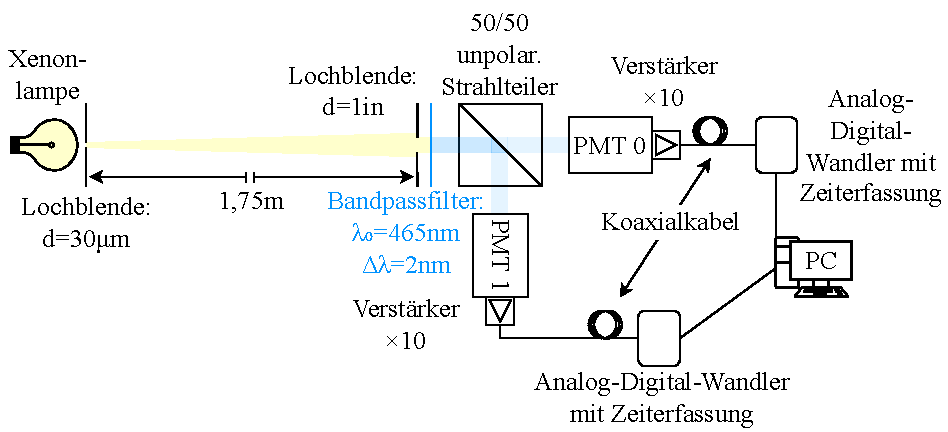
\includegraphics[width=0.9\linewidth]{images/Aufbau/Aufbau.pdf}
    \caption{Abgebildet ist eine vereinfachte Skizze des verwendeten Aufbaus, welche die konzeptuell wichtigsten Bauteile darstellt.}
    \label{fig:Versuchsaufbau}
\end{figure}
\todo{Fix Größe des Bildes, fontsize, abstand von pinhole hinzufügen}
Als Lichtquelle wird eine Xenon Lampe gewählt. 
Als Gasentladungslampe emittiert diese nach \autoref{ssec:Intensitäteninterferometrie} chaotisches Licht, welches bunching aufweist. 
Da nach dem van Cittert-Zernike Theorem der Winkeldurchmesser der Lichtquelle invers proportional zur Breite von $g^{(2)}(\bm{\rho})$ ist, ist weiterhin darauf zu achten die Ausdehnung der Lichtquelle einzuschränken, damit überhaupt korrelierte Photonen am Detektor vorliegen. 
Zu diesem Zweck ist eine kreisförmige Lochblende mit einem Durchmesser von $d=30\,\mathrm{\mu m}$ verbaut. 
Mit der Distanz $x=1,75\,\mathrm{m}$ zwischen Lichtquelle und dem restlichen Aufbau ergibt sich so ein Winkeldurchmesser von $\Delta \theta \approx \frac{d}{x} = 3,53\,\mathrm{asec}$. 
Es sei darauf hingewiesen, dass die größten Winkelsurchmesser von Sternen im Bereich von tausendstel Bogensekunden liegen \cite{hanburybrownAngularDiameters321974}, also etwa drei Größenordnungen kleiner sind, als der hier geschaffene \glqq künstliche Stern\grqq. \\
Um dem eintretenden Lichtstrahl eine definierte Breite zu geben, wird vor dieser zusätzlich durch eine Lochblende mit einem Durchmesser von einem Zoll geleitet. 
\todo{warum?}
Wie in \autoref{ssec:Michelson Sterninterferometer} beschrieben, ist für eine Messung der räumlichen Kohärenz auch eine nicht verschwindende Kohärenzzeit relevant. 
Da diese indirekt proportional zu spektralen Breite der Quelle ist, wird an dieser Stelle ein enger Bandpassfilter mit einer annähernd rechteckförmigen Transmissivität verbaut. 
Dieser hat nach Herstellerangaben eine zentrale Wellenlänge von $\lambda_0 = 465\,\mathrm{nm}$ und eine Breite von  $\Delta\lambda = 2\,\mathrm{nm}$ \cite{4652OD4Ultra}. 
Anschließend wird der Strahl durch einen nicht polarisierenden 50/50 Strahlteilerwürfel aufgeteilt und zum Nachweis der Photonen auf zwei Photomulitplier (PMTs) gelenkt. 
Direkt am Ausgang der Photomulitplier werden die Pulse mit einem Verstärker um den Faktor 10 verstärkt. 
Anschließend werden die Signale durch variable Kombinationen an Kabellänge und -modell zu Analog-Digital Wandlern (ADCs) geleitet, wo diese digitalisiert werden. 
Aufgrund des von Natur aus geringen Signals, werden alle analogen Signale durch geschirmte Koaxialkabel geleitet, um das Einkoppel von Störsignalen zu erschweren. 
Die Zeiterfassung der einzelnen ADC-Werte zur späteren Korrelation erfolgt durch Verwendung des White Rabbit Systems (vgl. z.B. \cite{lipinskiWhiteRabbitPTP2011}), welches direkt mit den ADCs verbunden ist. 
Abschließend werden die Daten am PC zur späteren Korrelation gespeichert. \\

Aufgrund des speziellen Aufbaus ergeben sich einige Änderungen bezüglich der im vorangegangenen Abschnitt eingeführten Theorie. 
Auf diese soll hier eingegangen werden. 
Wie erwähnt ist der Winkeldurchmesser der Quelle vergleichsweise groß. 
Nach \autoref{eq:erste nulstelle von g2(rho) für lochblende} wird für die Distanz zur ersten Nullstelle der $g^{(2)}$-Funktion lediglich $\rho_0\approx3,3\,\mathrm{cm}$ erwartet. 
Das heißt, dass am Beobachtungsort lediglich in einem Kreis mit Radius $\rho_0$ korrelierte Photonen auftreten. 
Aufgrund der physischen Größe der PMTs ist es daher nicht möglich, $g^{(2)}(\rho)$ für verschiedene $\rho$ zu messen. 
Stattdessen wird $g^{(2)}$ in einem Intervall $\rho\in[0,1]$ Zoll gemessen. 
Dieses entspricht den Abständen, die korrelierte Photonen durch die Lochblende am Eingang des Strahlteilers haben können. 
Es wird also erwartet, einen erniedrigten Wert für $g^{(2)}(\rho)$ und damit $\tau_c$ zu messen. 
Dies ist in \autoref{fig:räumliche koh simulation} verdeutlicht. 
Um herauszufinden, um welchen Faktor die gemessene Amplitude von der theoretischen maximalen Amplitude abweicht, wird eine Simulation durchgeführt, die sowohl den Wert von $g^{(2)}$ für jeden Photonenabstand als auch die Wahrscheinlichkeit für diesen berücksichtigt. 
Dieser Faktor beträgt bei gegebenem Aufbau $k_s=0,62$. 
\todo{Wie zitiere ich diese Simulationen?}
\begin{figure}[htbp]
    \centering
    \includegraphics{images/Aufbau/g2(rho).pdf}
    \caption{Dargestellt ist links die $g^{(2)}$-Funktion, abhängig von der Separation $\rho$. Rechts ist das Ergebnis der Simulation abgebildet. In blau ist $g^{(2)}$ für jeden Photonenabstand dargestellt (dies entspricht der Kurve im linken Graphen), während in orange die simulierte Wahrscheinlichkeitsverteilung ein Photoenpaar bei gegebenen Abstand anzutreffen aufgetragen ist. Durch Multiplikation der beiden Kurven erhält man den Faktor, um welchen die räumliche Kohärenz verringert ist. Dieser beträgt $k_s=0,62$. Links ist zudem eingezeichnet, welchem $\rho\prime$ eine Verringerung um ebendiesen Faktor entsprechen würde. }
    \label{fig:räumliche koh simulation}
\end{figure}
\todo{Verstehe ich es richtig, dass g2 um ks verringert wird? D.h. g2-1 liegt bei 2*ks -1 nicht bei ks???}
Über den theoretischen Verlauf der Korrelationsfunktion lässt sich durch $k_s$ auf einen effektiven Teleskopabstand $\rho\prime$ schließen, bei dem ein infinitesimal dünner Strahl den selben Verlust an räumlicher Kohärenz aufweist. 
Dies ist auch in \autoref{fig:räumliche koh simulation} veranschaulicht. \\
Aus voriger Überlegung ist nun bekannt $\tau_c^{meas} = k_s\cdot\tau_c^{th}$. 
Um $\tau_c^{th}$ zu bestimmen wird eine weitere Simulation verwendet. 
Diese berechnet aus dem vom Hersteller gegebenen Transmissionsprektrum des Filters über das Wiener-Khintchine Theore, d.h. eine Fouriertransformation die erwartete $g^{(1)}$-Funktion, welche anschließen über die Siegert-Relation in $g^{(2)}(\tau, \rho=0)$ umgerechnet wird. 
Daraus folgt dann für den vorliegenden Fall $\tau_c^{th} = \int g^{(2)}(\tau, \rho=0) -1 = 0,152\,\mathrm{ps}$. 
Abschließend ergibt sich also für die erwartete Kohärenzzeit bei dem verwendeten Aufbau:
\begin{equation}
    \tau_c^{meas} = 0,152\,\mathrm{ps}\cdot 0,62 = 94\,\mathrm{fs}
\end{equation}



\clearpage

\section{Datenaufnahme und Pre-Processing}
\label{sec:Datenaufnahme und Pre-Processing}
In diesem Abschnitt soll auf die Datenaufnahme sowie alle nötigen Schritte der Datenverarbeitung bis zur fertigen $g^{(2)}(\tau)$-Funktion eingegangen werden. 
Dafür werden zuerst die Datenaufnahme und dafür nötige Kalibrationsverfahren erläutert. 
In diesem Zuge wird zudem auf das Aussehen der aufgenommenen Daten eingegangen. 
Anschließend werden korrelierte Einzeldateien betrachtet und es wird verdeutlicht, warum eine Mittelung über viele Einzeldateien unumgäglich ist. 
Zuletzt werden angewandte Korrekturen und Filter angesprochen sowie verdeutlicht, wie die Mittelung der Daten erfolgt. 

\subsection{Datenaufnahme und Waveforms}
\label{ssec:Datenaufnahme und Waveforms}
Die Aufnahme der Daten erfolgt durch ein von der Arbeitsgruppe geschriebenes Programm, welches mit den ADCs kommuniziert. Ein Screenshot der GUI, auf dem die wichtigsten Schritte der Datenaufnahme markiert sind, ist in \autoref{fig:Screenshot GUI} eingefügt. 
\begin{figure}[h]
    \centering
    \includegraphics[width=0.9\textwidth]{images/Datenaufnahme/GUI.pdf}
    \caption{Dargestellt ist ein Screenshot der GUI zur Datenaufnahme. Wichtige Schritte sind markiert.}
    \label{fig:Screenshot GUI}
\end{figure}
In der GUI wird für jede verwendete Digitalisierungskarte ein Fenster erstellt, in dem Einstellungen für die jeweilige Karte vorgenommen werden können. 
Nach dem Erstellen eines Projekts können in dem mit \emph{1} markierten Bereich in \autoref{fig:Screenshot GUI} Einstellungen für die ADC-Karte vorgenommen werden. 
Es wird mit einem Kanal je Karte gemessen und die Samplingzeit beträgt $1{,}6$\,ns bei einer Dateigröße von 2 Gigasamplen. 
Der zu digitalisierende Spannungsbereich wird auf 200\,mV gesetzt, sodass die in \emph{4} abgebildeten Waveforms den dargestellten Digitalisierungsbereich von $-128\,\mathrm{ADC}$ nicht überschreiten. 
Clock und Trigger werden extern durch das White Rabbit System gegeben. 
Die genannten Einstellung werden größtenteils vor der Messung automatisch mit dem Button \glqq Init new measurement\grqq\;gesetzt. \\
Vor Start der Messung müssen zwei Kalibrationsschritte für jeden Kanal gemacht werden. 
Zuerst wird unter \emph{2} eine Offset-Messung durchgeführt, indem \glqq Measure\grqq\;und \glqq Calc Offset\grqq\;gewählt werden. 
Diese wird ohne Beleuchtung und mit ausgeschalteter Hochspannung durchgeführt. 
Das Programm bestimmt diesen vom Verstärker abhängigen Offset und speichert diesen zur späteren Entfernung \cite{zmijaOpticalIntensityInterferometry2021}. 
Anschließend wird bei eingeschalteter Hochspannung und niedriger Photonenrate eine PMT-Puls-Kalibration durchgeführt, sodass gemessene Spannungen in Photonenraten umgerechnet werden können. 
Die Kalibration ist nötig, da aufgrund der hohen Raten bei der Messung keine Einzelphotonenpulse vorliegen, aus denen sich die Raten einfach bestimmen lassen würden, sondern die Pulse überlappen.
Für die Kalibration wird für jeden Kanal die mittlere Pulsform der PMT-Pulse bestimmt und gespeichert, woraus anschließend eine druchschnittliche Ladung pro Puls und damit die Rate berechnet werden kann.
Die Ratenanzeige in \emph{5} ist nützlich zur leichteren Justierung des optischen Aufbaus (Maximierung der Rate), sowie bei der Beobachtung eines Sterns zum Vergleich mit Theoriewerten.
Für die vorliegende Arbeit ist allerdings hauptsächlich relevant, dass während der Kalibration die mittlere PMT-Pulsform gespeichert wird.
Es wird erwartet, dass diese einen bedeutenden Einfluss auf die Form der $g^{(2)}$-Funktion hat, da die Photonenpulse deutlich breiter sind als die einzelnen $1{,}6$\,ns-Bins, was zu einer Korrelation benachbarter Bins führt \cite{zmijaOpticalIntensityInterferometry2021}. 
Aus den gemessenen Daten wird bestimmt, wie viel Ladung ein Photon, das auf einen PMT trifft, durchschnittlich freisetzt, woraus anschließend die in \emph{5} gezeigten Photonenraten in MHz bestimmt werden können. \\
Nach diesen Kalibrationsschritten kann die Messung gestartet werden, woraufhin synchronisiert durch den Trigger des White Rabbit Systems 2$\cross$2\,GS Daten aufgenommen werden. 
Dies entspricht einer Messdauer von $3{,}436\,\mathrm{s}$. 
Nach Ablauf von 4\,s startet anschließend der nächste Trigger eine Messung von 2$\cross$2\,GS, sodass idealerweise ein Duty-Cycle von 85{,}9\% erreicht wird \cite{zmijaFirstIntensityInterferometry2023}. 
Da jedes Sample einem 8\,bit ADC-Wert entspricht, erreicht die Messung also eine Datenrate von 2$\cross$2\,GB alle 4\,s, was erklärt, weshalb die Daten erst gespeichert und anschließend offline korreliert werden. 
Zur Veranschaulichung ist in \autoref{fig:Offest_Rate Kalibration} aufgezeigt, wie eine typische Waveform zur Offset-Messung, Puls-Kalibration und zur Messung aussieht. 
\begin{figure}[h]
    \centering
    \includegraphics{images/Datenaufnahme/Kalibration.pdf}
    \caption{Abgebildet ist der Ausschnitt einer Waveform für die Offset-Messung in Orange (ausgeschaltete Hochspannung und Beleuchtung), Puls-Kalibration in Blau (Hochspannung und Licht an, niedrige Photonenrate) und für die Messung in Grau.}
    \label{fig:Offest_Rate Kalibration}
\end{figure}

\subsection{Korrelation}
\label{ssec:Korrelation}
Die Korrelation der Daten erfolgt parallelisiert, nachdem die Datenaufnahme abgeschlossen ist. 
Jede Datei von beiden Kanälen wird getrennt miteinander korreliert, indem diese zuerst in Vektoren $\mathbf{A}$ und $\mathbf{B}$ eingelesen werden. 
Anschließend wird für jede Zeitdifferenz $\tau$ das folgende Skalarprodukt berechnet: 
\begin{equation}
    G^{(2)}(\tau) = \mathbf{A}(t)\cdot\mathbf{B}(t+\tau)
    \label{eq:korrelation}
\end{equation}
Damit entspricht jeder Wert von $G^{(2)}(\tau)$ der unnormierten zeitlichen Photonenkorrelation zu diesem Zeitpunkt \cite{zmijaOpticalIntensityInterferometry2021}. 
Die korrelierten Einzeldateien können anschließend für die weitere Datenanalyse gespeichert werden, da diese deutlich kleiner (im Bereich weniger kB) sind als die Rohdaten. 
Um aus einer bestimmten $G^{(2)}$-Funktion die normierte zeitliche Korrelationsfunktion zu erhalten, wird diese durch ihren Mittelwert weit außerhalb des Bunching Peaks geteilt:
\begin{equation}
    g^{(2)}(\tau) = \frac{G^{(2)}(\tau)}{\overline{G^{(2)}(\tau\gg\tau_{\mathrm{c}})}}
    \label{eq:G2 normalisierung}
\end{equation}
Ein Beispiel für die unnormierte Funktion $G^{(2)}$ einer einzelnen Datei ist in \autoref{fig:G2(tau)} dargestellt. 
\begin{figure}[h]
    \centering
    \includegraphics{images/Datenaufnahme/G2.pdf}
    \caption{Ein Beispiel einer unnormierten Korrelationsfunktion ist abgebildet. Durch das verrauschte Signal ist an der Stelle $\tau=0$ kein Bunching Peak sichtbar.}
    \label{fig:G2(tau)}
\end{figure}
Es ist ersichtlich, dass die Funktion stark verrauscht ist und der Bunching Peak nicht auszumachen ist. 
Die in \autoref{ssec:Intensitätsinterferometrie} bereits erwähnte Notwendigkeit der Mittelung über viele Daten, d. h. lange Zeiten, um die Form von $g^{(2)}$ bestimmen zu können, ist daher deutlich sichtbar. 

\subsection{Mittelung der Daten und Filter}
\label{ssec:mittelung und filter}
Wie bereits im vorangegangenen Abschnitt ersichtlich wurde, ist eine Mittelung vieler Dateien unumgänglich, um den Bunching Peak analysieren zu können. 
Hierbei wird der Ansatz eines gewichteten Mittelwerts gewählt, da nicht jede der etwa $3{,}4\,\mathrm{s}$ langen Dateien statistisch gleich aussagekräftig ist. 
So weisen manche der Messabschnitte höhere Photonenraten auf als andere (vgl. dazu \autoref{fig:Screenshot GUI}, Kasten \emph{5}). 
Unter der Annahme, dass ein Großteil des Rauschens in der $G^{(2)}$-Funktion statistischen Fluktuationen entspricht, wird erwartet, dass das Rauschen für höhere Photonenraten abnimmt. 
Dies bedeutet, dass Dateien mit höheren Raten und geringerer Schwankung stärker gewichtet werden sollten, als jene mit geringeren Photonenraten. 
Um dies zu bewerkstelligen, wird von jeder Datei $G^{(2)}_i$ die Standardabweichung $\sigma_i$ bestimmt und anschließend der folgende gewichtete Mittelwert berechnet \cite{cochranProblemsArisingAnalysis1937}:
\begin{equation}
    \overline{G^{(2)}} = \frac{\sum_{i=0}^{n}\frac{G^{(2)}_i}{\sigma_i^2}}{\sum_{i=0}^{n} \sigma_i^{-2}}
\end{equation}
Das Ergebnis der Mittelung über 10000 Dateien, d. h. etwa $9{,}5$\,h Korrelationsdaten, ist in \autoref{fig:gemittelte G2 vs g2} oben abgebildet. 
Der Bunching Peak bei $\tau\approx 0$ ist nach Mittelung der Daten bereits sichtbar. 
Allerdings sind durch die Mittelung weitere Artefakte ersichtlich geworden. 
Bereits in den korrelierten Einzeldateien ist eine Struktur in den Daten zu erkennen, welche das Signal überlagert. 
Nach der Mittelung ist diese nun besonders deutlich, was darauf hinweist, dass sie nicht von rein statistischer Natur ist, sondern tatsächlich zwischen den Kanälen korreliert ist. 
Das etwa $12\,\mathrm{\mu s}$ breite Störsignal wird von der Spannungsversorgung der Xenonlampe erzeugt \cite{zmijaOpticalIntensityInterferometry2021}, liegt daher in beiden Kanälen zugleich vor und wird deshalb durch die Korrelation und Mittelung verstärkt. 
Da es aber mehrere Größenordnungen breiter ist als der Bunching Peak und diesen daher kaum beeinflusst, wird es in diesem Abschnitt erst einmal vernachlässigt. 
In einem späteren Abschnitt zur Integration des Peaks wird auf eine Methode eingegangen, dieses Störsignal zu entfernen. \\
\begin{figure}[h]
    \centering
    \includegraphics{images/Datenaufnahme/G2_vs_g2.pdf}
    \caption{Dargestellt ist der Unterschied zwischen $G^{(2)}(\tau)$ (oben) und der normierten Funktion $g^{(2)}(\tau)$ nach Mittelung über 10000 Dateien (unten), bei der zudem die \glqq pattern correction\grqq\;und der Tiefpass angewandt worden sind. Es ist deutlich erkennbar, dass die angewandten Methoden zu einer starken Verbesserung des Signal-Rausch-Verhältnisses geführt haben. }
    \label{fig:gemittelte G2 vs g2}
\end{figure}
Weiterhin ist durch Zoom in die Daten oder eine Fouriertransformation dieser ein 8-Bin-periodisches Muster zu erkennen, welches dafür verantwortlich ist, dass die $G^{(2)}$-Funktion ein breites Band an Werten annimmt. 
Dieses von den ADC-Karten kommende Muster stört den Verlauf des Bunching Peaks in beträchtlicher Weise, da es sich auf der selben Zeitskala wie der Peak selbst befindet. 
Da das Störsignal von den beiden ADC-Karten gleichzeitig ausgeht, ist dieses korreliert und daher besonders dominant in der abgebildeten $G^{(2)}$-Funktion.
Um das Störsignal zu entfernen, wird eine von der Arbeitsgruppe geschriebene \glqq pattern correction\grqq\;angewandt, welche in den ersten 4000 Bins (d. h. im Intervall $\tau\in[-8000,-1600]\,\mathrm{ns}$) jeweils 8 Bins mittelt und die Daten anschließend durch das so ermittelte Muster teilt. 
Da das Muster sowohl das eigentliche 8-Bin-periodische Muster, als auch den Offset der $G^{(2)}$-Funktion (vgl. \autoref{eq:G2 normalisierung}) enthält, wird diese durch die Division automatisch auch normiert. 
Der Schritt der \glqq pattern correction\grqq\;wird für jede Datei separat vor der Bildung des Mittelwertes angewandt. \\
Nach diesen Schritten wird auf die gemittelte $g^{(2)}$-Funktion noch ein digitaler Tiefpass 2. Ordnung mit einer Grenzfrequenz von 200\,MHz angewandt, um weitere hochfrequente Störsignale zu entfernen. 
Die nach erwähnten Korrekturen und der angewandten Mittelung erhaltene Funktion $g^{(2)}(\tau)$ ist in \autoref{fig:gemittelte G2 vs g2} unten abgebildet. 


\clearpage
%---------------------------------------------------------
%	Acronyms
%---------------------------------------------------------

% \clearpage
% \mbox{}
% \clearpage
% \printnoidxglossary[type=acronym]
% \printacronyms
% \clearpage

%---------------------------------------------------------
%	Appendix (if needed)
%---------------------------------------------------------
% \clearpage
% \mbox{}
% \clearpage
% \appendix
% \addtocontents{toc}{\protect\setcounter{tocdepth}{1}}
% \addtocontents{toc}{\protect\renewcommand{\protect\sectionautorefname}{Appendix}}
% \newgeometry{
% 	%a4paper,
% 	left=40mm,
%     % right=20mm,
% 	top=15mm,
% }
%     
\section{Appendix A}
Your appendix goes here!



%---------------------------------------------------------
%	Bibliography
%---------------------------------------------------------

\clearpage
\mbox{}
\clearpage

\newgeometry{
	%a4paper,
	left=40mm,
    % right=20mm,
	top=35mm,
}
\renewcommand\refname{Bibliography}
% \printbibliography
\printbibliography[
heading=bibintoc,
title={Bibliografie}
]

%---------------------------------------------------------
%	Danksagung
%---------------------------------------------------------

% \clearpage
% \mbox{}
% \clearpage

% \section*{Danksagung}
Here you can thank everyone you want to. 
% 
\begin{itemize}
    \item Max Mustermann for having a name that is simple to remember.
    \item Dr. Albert Einstein for having fun ideas about space-time.
\end{itemize}


% \clearpage
%---------------------------------------------------------
%	Eigenständigkeitserklärung / Declaration of independence
%---------------------------------------------------------

% \selectlanguage{german}
% \section*{Eigenständigkeitserklärung}
% Hiermit versichere ich, Stephen Weybrecht (22967286), die vorgelegte Arbeit selbstständig und ohne unzulässige Hilfe Dritter sowie ohne die Hinzuziehung nicht offengelegter und insbesondere nicht zugelassener Hilfsmittel angefertigt zu haben. Die Arbeit hat in gleicher oder ähnlicher Form noch keiner anderen Prüfungsbehörde vorgelegen und wurde auch von keiner anderen Prüfungsbehörde bereits als Teil einer Prüfung angenommen.\\

% Die Stellen der Arbeit, die anderen Quellen im Wortlaut oder dem Sinn nach entnommen wurden, sind durch Angaben der Herkunft kenntlich gemacht. Dies gilt auch für Zeichnungen, Skizzen, bildliche Darstellungen sowie für Quellen aus dem Internet.\\

% Mir ist insbesondere bewusst, dass die Nutzung künstlicher Intelligenz verboten ist, sofern diese nicht ausdrücklich als Hilfsmittel von dem Prüfungsleiter bzw. der Prüfungsleiterin zugelassen wurde. Dies gilt insbesondere für Chatbots (insbesondere ChatGPT) bzw. allgemein solche Programme, die anstelle meiner Person die Aufgabenstellung der Prüfung bzw. Teile derselben bearbeiten könnten.\\

% \vspace{10cm}
% \begin{flushleft}
% \makebox[.4\textwidth]{\hrulefill}\hfill \makebox[.4\textwidth]{\hrulefill}\\
% \makebox[.4\textwidth]{Ort, Datum}\hfill
% \makebox[.4\textwidth]{Unterschrift}\\
% \end{flushleft}


\end{document}

